\chapter{Introduction}
\label{chap:Introduction}

Optical music recognition (OMR) is an~interesting subfield of computer vision. It shares a~lot of similarities to optical character recognition (OCR) and handwritten text recognition (HTR). It is, however, more challenging as is pointed out in the~paper \emph{Understanding Optical Music Recognition} (\cite{CalvoZaragozaHajic}). For~example in OCR, characters are read in one direction, typically from left to right. Musical symbols seem to be similar in that a~staff is also read from left to right, but many symbols can be placed above each other. Piano scores can even have symbols that span multiple staves.

Although a~musical score can be very complex, many scores are not. We can limit ourselves to scores that are monophonic, have a~single voice, and have symbols spanning only one staff. Monophonic scores lack chords, meaning there is only one note playing at a~time. This holds, for example, for windblown instruments, since they cannot play multiple notes simultaneously. Sometimes multiple voices (instruments) are engraved in a~single staff to save space. We will not attempt to read these scores either. It would be like reading two lines of text simultaneously and the proposed model can output only a~single sequence. Also deciding what voice a~given note belongs to is in itself a~complicated problem.

Deep neural networks have transformed the field of computer vision recently. Especially convolutional networks (CNN), whose architecture is particularly well suited for image processing. Recurrent neural networks (RNN) have been used for sequence processing, like natural language modeling or natural language translation. We can combine these two architectures to create a~so-called RCNN network. When trained using connectionist temporal classification (CTC), we get a~powerful architecture that is ideal for processing visual sequential data (\cite{Puigcerver}). This architecture has been used in handwritten text recognition to yield state-of-the-art results (\cite{Scheidl}).

If we limit the~complexity of musical scores to the point that a~single staff can be represented as a~sequence of tokens, we can use this architecture to tackle the problem of OMR. This approach has been tried in 2018 by Calvo-Zaragoza and Rizo (\cite{Primus}). They created the PrIMuS dataset, which contains 87678 real-music incipits. An~incipit is the part of a~melody or a~musical work that is most recognizable for that work. Each incipit is a~few measures long, typically shorter than a~single staff of printed sheet music would be.

The resulting model has been compared against Audiveris\footnote{\href{https://github.com/Audiveris}{https://github.com/Audiveris}}, an~open-source OMR tool, and has proven to be superior on the~PrIMuS dataset. However, the~dataset contains printed images only. Since this RCNN architecture is an~end-to-end approach, there is a~great chance that it would be ideal for reading handwritten scores as~well (drawing analogy from HTR).

Therefore the goal of this thesis is to explore the~end-to-end approach for optical music recognition of handwritten music scores. More specifically we want to train an~RCNN network to yield the best possible results on the~CVC-MUSCIMA dataset.

\overfullrule=0pt % fixes black rectangle issue
We needed to obtain training data. We explored the \emph{Collection of datasets for OMR} by~Alexander Pacha (\cite{Pacha}) and quickly found out that the~only dataset containing entire staves of handwritten sheet music is the~CVC-MUSCIMA dataset (\cite{CvcMuscima}). Every other handwritten dataset contains only musical symbols or is derived from CVC-MUSCIMA. Since CVC-MUSCIMA is intended for writer classification and staff removal, it contains only 20 parts, each written by 50 writers. That is far too small variability, given the~task we are trying to solve.

Facing this issue we resorted to data augmentation. The~idea is to take handwritten musical symbols and place them onto an~empty staff to create a~new staff image. We called this music engraving system \emph{Mashcima} and the~system is explained in chapter \ref{chap:EngravingSystem}. The~musical symbols used by~Mashcima come from the~MUSCIMA++ dataset (\cite{MuscimaPP}). This~dataset is built on top of CVC-MUSCIMA and provides pixel-perfect symbol segmentation and relationships between symbols. The~reason we choose MUSCIMA++, instead of other musical symbol datasets, is that it is built on top of CVC-MUSCIMA. This means the~image resolution and overall style are consistent with CVC-MUSCIMA. Also, MUSCIMA++ has been developed at~Charles University and~so it was easy to contact its creator when needed. We however do make sure, that the~final evaluation is performed on data the~neural network has not seen during training. Specifically, it trains on staves by completely different writers than the~ones used for evaluation.

Mashcima engraving system is the~main feature that sets this thesis apart from other works. Other people, when faced with the~lack of training data, used data augmentation (dilation, blurring, distortion) or transfer learning (\cite{HmrBaseline}). We believe that a~custom engraving system for handwritten music is the~best way to produce an~overabundance of high-quality training data. Our confidence stems from the fact, that non-trained human has difficulties distinguishing a~real-world sample from a~well-engraved one (see Figure \ref{fig1:Comparison}).

\begin{figure}[h]
    \centering
    \setlength{\unitlength}{1.0cm}
    \begin{picture}(14,6.5)
        %\thicklines
        %\put(0,0){\line(1,0){14}}
        %\put(0,0){\line(0, 1){6.5}}

        \put(0.5,3.5){
            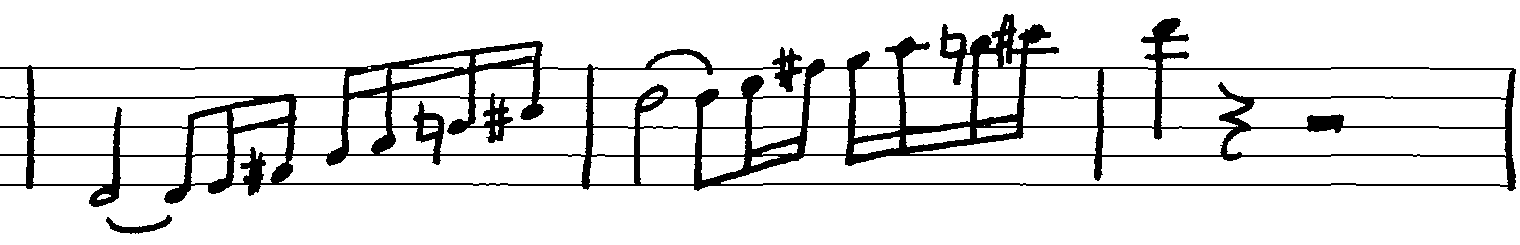
\includegraphics[width=130mm]{../img/comparison-real}
        }
        \put(0,0){
            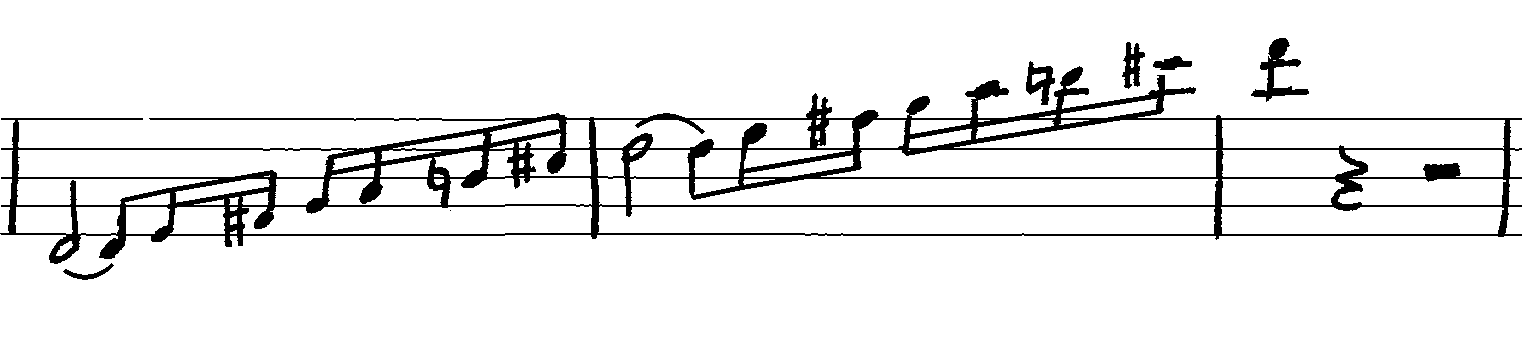
\includegraphics[width=140mm]{../img/comparison-engraved}
        }

        \put(0,5.8){\texttt{Real-world:}}
        \put(0,2.8){\texttt{Synthetic:}}
    \end{picture}
    \caption{
    Comparison of a real-world image to an engraved image. The top image is taken from the CVC-MUSCIMA dataset. The bottom image is the same music engraved using our engraving system and using symbols of the same writer.
    }
    \label{fig1:Comparison}
\end{figure}

It is difficult to evaluate an~OMR~system in general. This is because there is no standard dataset that can be used and no standard set of metrics. Moreover, we proposed a~new Mashcima representation for the music engraved in a~staff. This representation is based on the~agnostic encoding proposed by Calvo-Zaragoza and Rizo (\cite{Primus}). Using custom representation makes it yet more difficult to compare our results to other works. That being said, we can still make some comparisons. It seems that having a~specialized engraving system is a~step in the right direction. The results we obtained when evaluating are comparable to similar works performing similar evaluation (\cite{HmrBaseline}).

The~thesis assignment states that the~output of our model will be a~MusicXML file. We quickly realized that the~problem is far larger than anticipated and so we focused on the~core features only. Similarly, the~model input is not a~plain photo or scan. It is already preprocessed and binarized. This problem has already been solved during the~creation of the~CVC-MUSCIMA dataset (\cite{CvcMuscima}), therefore we did not tackle it either.

Also, there is a~Github repository containing all the~source code and text of this thesis at \href{https://github.com/Jirka-Mayer/BachelorThesis}{\texttt{https://github.com/Jirka-Mayer/BachelorThesis}}. There is also a~release tag corresponding to the~time this thesis was submitted and it contains all the~trained models for download.

\section{Thesis Outline}

\paragraph{Chapter \ref{chap:Introduction}:} This chapter provides an introduction to the problem this thesis attempts to solve. It describes the approach we tried and how successful it was.

\paragraph{Chapter \ref{chap:RelatedWork}:} This chapter lists work done by other people that we build upon and that will be referenced throughout the thesis. It provides a short overview of each work and of what significance it is to us.

\paragraph{Chapter \ref{chap:DeepNeuralNetwork}:} This chapter describes the specific model we decided to use for our OMR task. It discusses traditional methods and how deep neural networks help us simplify the process. It describes models other people used for similar tasks and how we have been influenced by them.

\paragraph{Chapter \ref{chap:MusicRepresentation}:} This chapter mainly describes the Mashcima music encoding - the encoding we used for our model. It describes how it relates to the PrIMuS agnostic encoding, and why we made certain decisions regarding its design.

\paragraph{Chapter \ref{chap:EngravingSystem}:} This chapter talks about the Mashcima engraving system. Why we developed this system and what problem it solves. How it works, what are its limitations, and how it can be extended.

\paragraph{Chapter \ref{chap:ExperimentsAndResults}:} This chapter describes the experiments we performed. These experiments aim to measure the performance of our approach and test hypotheses postulated in previous chapters. We will also attempt to compare our results to other similar works.
